% Intro paragraph. 1 sentence on why the topic, why is it challenging, what this thesis does, outline of the chapter
With the recent increase in capability of autonomous systems, they are being deployed in safety-critical domains such as autonomous driving, aviation, and medicine where the consequences of operational errors include loss of property or human life. Ensuring the safe operation of safety-critical autonomous systems is a necessary step before deployment, but remains a significant technical challenge due to the complexity of systems and the environments in which they operate. This thesis presents scalable, interpretable, and efficient methods for validating the safety of autonomous systems in simulation. This chapter first discusses the general problem of autonomous system safety and argues that safety validation through black-box sampling plays a crucial role. The next sections goes on to give an overview of the challenges of black-box to safety validation approaches, followed by the contributions and outline of the thesis. 

\section{Safety Validation of Autonomous Systems}

% Why should we want autonomous systems
Introducing autonomy into safety-critical domains has the potential to improve both safety and efficiency. Driving accidents killed \num{1.35} million people in 2016~\cite{world2019global}, and approximately \num{94}\% of accidents between 2005--2007 in the US were due to driver error~\cite{singh2015critical}. Autonomous aircraft collision avoidance systems were put into place after a series of devastating mid-air collisions~\cite{federal2011introduction} and have been shown to reduce the (already rare) risk of mid-air collision by at least a factor of 3~\cite{arino2002studies}. The next generation of aircraft collision avoidance systems will improve safety and function in the higher-density airspaces in the future~\cite{kochenderfer2012next}.

% There are risks as well
Although the upside of automation can be large, there are serious risks involved in deploying such systems. On March 18, 2018, a vehicle controlled by an autonomous system struck and killed a pedestrian in Arizona. A report of the incident found that the vehicle observed the pedestrian as an unknown object \num{6} seconds prior to the collision but failed to classify the pedestrian and gave varying predictions for the future path of travel. It took an additional \num{4.7} seconds for the autonomous system to determine that emergency braking was required~\cite{board2018preliminary}. Another example of risk comes from aircraft collision avoidance systems. Aircraft collision avoidance systems have the potential to induce a small number of mid-air collisions that would not have otherwise occurred~\cite{arino2002studies}. The number of induced collisions is much smaller than the number of prevented collisions, but these induced collisions highlight the possibility of bad outcomes for systems that are improperly designed, tested or deployed.

\begin{figure}[!t]
\centering
\resizebox{0.9\textwidth}{!}{%
\begin{tikzpicture}
% Arrows
\draw[fill=gray!20,line width=1pt] (144:\radius + \half) arc (144:72 + \stem:\radius+\half) -- (72 + \stem:\radius+\half+\head) -- (72 + \stem - \margin:\radius) -- (72+\stem:\radius-\half-\head) -- (72+\stem:\radius-\half) arc (72+\stem:144:\radius-\half)--cycle;

\draw[fill=gray!20,line width=1pt] (72:\radius + \half) arc (72:0 + \stem:\radius+\half) -- (0 + \stem:\radius+\half+\head) -- (0 + \stem - \margin:\radius) -- (0+\stem:\radius-\half-\head) -- (0+\stem:\radius-\half) arc (0+\stem:72:\radius-\half)--cycle;

\draw[fill=gray!20,line width=1pt] (0:\radius + \half) arc (0:-72 + \stem:\radius+\half) -- (-72 + \stem:\radius+\half+\head) -- (-72 + \stem - \margin:\radius) -- (-72+\stem:\radius-\half-\head) -- (-72+\stem:\radius-\half) arc (-72+\stem:0:\radius-\half)--cycle;

\draw[fill=gray!20,line width=1pt] (-72:\radius + \half) arc (-72:-144 + \stem:\radius+\half) -- (-144 + \stem:\radius+\half+\head) -- (-144 + \stem - \margin:\radius) -- (-144+\stem:\radius-\half-\head) -- (-144+\stem:\radius-\half) arc (-144+\stem:-72:\radius-\half)--cycle;

\draw[fill=gray!20,line width=0pt] (-144:\radius + \half) arc (-144:-216 + \stem:\radius+\half) -- (-216 + \stem:\radius+\half+\head) -- (-216 + \stem - \margin:\radius) -- (-216+\stem:\radius-\half-\head) -- (-216+\stem:\radius-\half) arc (-216+\stem:-144:\radius-\half)--cycle;


\node[nstyle, fill=c1!80, ] at (144:\radius) (test)
{
\includegraphics[height=2.\nsize]{figures/introduction/blueprint}};
\node[text width=8cm, anchor=west] at (-13cm, 4.4cm) {\setulcolor{c1} {\LARGE{\ul{\bf 1. Define Requirements}}} \\ 
\Large
\begin{itemize}
\item Temporal logic
\item Dangerous states
\end{itemize}
};

\node[nstyle, fill=c2!80] at (72:\radius) {
\includegraphics[height=2.\nsize]{figures/introduction/eng}};
\node[text width=8cm, anchor = west] at (3.6cm, 6cm) {\setulcolor{c2} {\LARGE{\ul{\bf 2. Design Effort}}} \\ 
\Large
\begin{itemize}
\item Machine learning
\item Engineering
\end{itemize}
};

\node[nstyle, fill=c3!80] at (0:\radius) {
\includegraphics[width=2.\nsize]{figures/introduction/tree}};

\node[text width=8cm] at (6:\radius + 6cm) {\setulcolor{c3} {\LARGE{\ul{\bf 3. Generate  Testcases}}} \\ 
\Large
\begin{itemize}
\item Unit tests
\item Automated testing
\end{itemize}
};

\node[nstyle, fill=c4!80] at (-72:\radius) {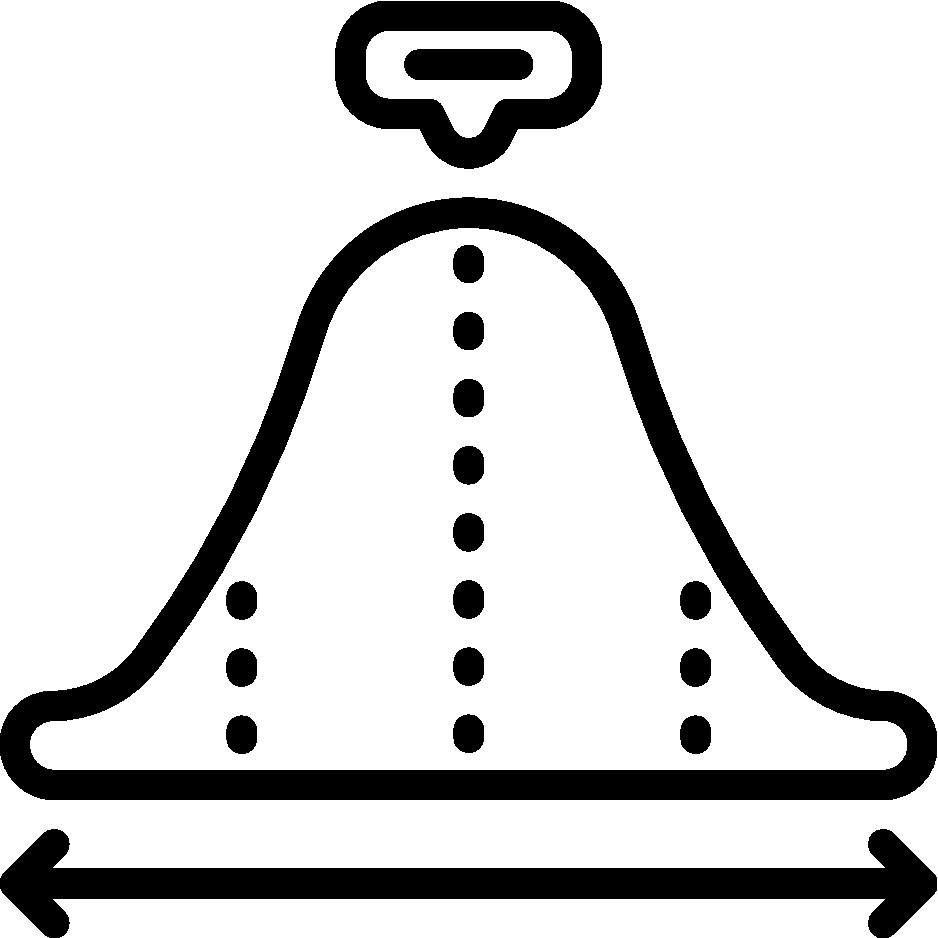
\includegraphics[height=2.\nsize]{figures/introduction/graph}};

\node[text width=10cm] at (-36:\radius + 6.2cm) {\setulcolor{c4} {\LARGE{\ul{\bf 4. Evaluate  Performance}}} \\ 
\Large
\begin{itemize}
\item Failure probability
\item Failure severity
\end{itemize}
};


\node[nstyle, fill=c5!80] at (-144:\radius) {
\includegraphics[height=2.\nsize]{figures/introduction/head}};

\node[text width=8cm,anchor=west] at (-13.5cm, -3.5cm) {\setulcolor{c5} {\LARGE{\ul{\bf 5. Interpret Failures}}} \\ 
\Large
\begin{itemize}
\item Failure classification
\item Root cause analysis
\end{itemize}
};
\end{tikzpicture}
}
\caption{The design cycle of an autonomous system.  }
\label{fig:design_cycle}
\end{figure}

% Description of the design cycle of an autonomous system
To understand how to incorporate safety into autonomous system, we must first understand how such systems are designed. The design cycle of autonomous systems is shown in \cref{fig:design_cycle}. The first step in system design is the \emph{definition of requirements} which may include specifications on performance, safety, interpretability, and more. Then, some \emph{design effort} is expended to develop a prototype of the system. Modern and future autonomous system design will usually involve a combination of machine learning and engineering. Once a prototype of the system is available, it must undergo \emph{testing} in the form of unit tests of specific components and integration tests of the larger subsystems. The generation of these test cases can be done from expert knowledge or can be automated. Based on the results of the tests, the system is \emph{evaluated} on any number of performance metrics. Safety metrics may include the probability the system violates its safety specification (referred to as a \emph{failure}) or the severity of observed failures. A this point, if the systems meets all required performance and safety specifications, it can be deployed. If not, then the failures of the system need to be \emph{interpreted} to discover discover broad categories of failures, called \emph{failure modes} and to perform root-cause analysis to discover flaws in the system. Once failures are identified and categorized, this may induce a change in the system requirements and the cycle continues until the system is ready for deployment. 


%Safety of an autonomous systems should be incorporated at all stages of the development
Safety can and should be incorporated at all stages of the design cycle. This thesis focuses primarily on \emph{safety validation}, which covers the stages of testing, performance evaluation and failure interpretation, but we will first briefly describe how safety can be included in the stages of requirement definition and design. 

The most straightforward why of including safety in the definition of system requirements is to identify what is meant by a failure and stipulate a maximum allowable failure probability or failure severity. Although this type of requirement provides a concrete safety goal, it does not necessarily help the design process more easily produce a safe system. A thorough analysis of the environment and system may allow for a set of specifications that can guarantee safety under a set of assumptions. For autonomous driving, the responsibility-sensitive safety model~\cite{shalev2017formal} and the safety force field model~\cite{nister2019safety} both develop a set of rules that restrict the actions of a driving agent to ensure safety. These specifications are not comprehensive enough to define a complete driving agent, but an agent based on machine learning may be trained to satisfy a goal while respecting such specifications~\cite{sadigh2014learning,bouton2019reinforcement}.

Designing a safe autonomous system with machine learning can be especially challenging. Approaches to improve safety of machine-learned systems include defining objectives that adequately penalize rare but catastrophic failures~\cite{moldovan2012risk} or are risk-aware~\cite{tamar2014policy}, learning from safe human demonstrations~\cite{abbeel2005exploration}, and training on adversarial examples~\cite{goodfellow2014explaining}. For agents that continue to learn in their operational environment, they will need to perform safe exploration which can be done by only allowing exploratory actions that are reversible~\cite{moldovan2012safe}, through active learning~\cite{garcia2013safe}, or through uncertainty-awareness~\cite{sui2015safe}. For a good overview on the topic of safe reinforcement learning see \textcite{garcia2015comprehensive} and \textcite{amodei2016concrete}. 


% Compare and contrast different techniques (Testing in the real world, scenario-based or unit tests, formal methods, black both approaches)
Safety validation is performed on an existing prototype of a system and can have several objectives. Safety can be used to discover failures of the system, compute the likelihood that the system fails, or to understand which environmental factors might lead to a system failure. There are many techniques that are used for safety validation, each with pros and cons. Below we discuss four categories of validation approaches. 

\paragraph{Scenario-based testing} Usually done in simulation, scenario-based testing is a form of unit testing where scenarios are developed to challenge specific behaviors or components of an autonomous system. These scenarios can be constructed from real-world data or through expert knowledge, and can be designed to focus on potential weaknesses of the system. Scenario-based testing can be used for regression testing, where the same suite of scenarios is applied to the system each time the system changes to make sure no failure modes have been introduced. The downside to scenario-based testing is the possibility of missing important failure cases because they were not included the suite of tests. Critical tests may be excluded due to incorrect assumptions about the environment or due to the difficulty of predicting failures caused by the complex interaction of many components.

\paragraph{Real-world testing} In real-world testing, a prototype of the system is used in an environment that is as close as possible to the intended deployment environment. For autonomous driving this may be a closed course or an area of a city that has already undergone extensive mapping. Usually, the system will be equipped with extra safety features to mitigate risk. This form of testing is critical before deployment because there may be complications that arise when moving from simulated environments to the real world. The downside to real-world testing is the high cost (in both time and other resources) and the high consequence if the system behaves unsafely.

\paragraph{Formal verification} Formal verification techniques can provide mathematical proofs about system safety under a set of assumptions. The system must first be described by a mathematical model such as a finite state machine, computer code, or the parameters and architecture of a neural network. The model is checked against a safety specification usually written in a temporal logic. In \emph{model checking} all inputs to the system are exhaustively checked to discover any outputs that violate the safety specification. If there are no violations, then the system is concluded to be safe. Another approach is \emph{deductive verification} where a proof of safety is constructed through a series of intermediate theorems about the behavior of the system. These proofs are often constructed with automated theorem provers. Formal verification gives the highest degree of confidence in the safety of a system under the assumption that the mathematical model adequately represents the true system. The main drawback to formal verification is that it may not scale well to systems with large or continuous state spaces operating in environments with a large number of inputs to the system. 

\paragraph{Black-box sampling and learning} Black-box sampling techniques involve repeatedly simulating the system in a stochastic model of the environment to discover failures. The term \emph{black-box} comes from the assumption that we do not know anything about the structure of the system and can only interact with it through inputs and outputs. This assumptions allows black-box sampling approaches to be applied to complex systems. In the case where failures are rare, random simulation may be inefficient for finding failure examples or computing the probability of failure. In this case, learning techniques can be applied to iteratively improve the stochastic parameters of the environment to make failures more likely to occur. The downside to black-box sampling techniques and learning is that we will never be fully confident in the safety of the system, and instead must rely on probabilistic conclusions of safety. 

While all of the safety validation approaches are useful in different circumstances, we focus on black-box safety validation due to its favorable scalability and the ease with which it can be combined with powerful machine learning algorithms.


\section{Challenges to Black-Box Safety Validation}
There are many challenges for algorithms that use black-box sampling including accurate modeling of the system and the environment, efficiency in the number of simulations required, and interpretability of discovered failures. 

% Challenges of modeling the system and environment
Although not discussed in detail in the rest of this thesis, the challenge of accurately modeling an autonomous system interacting with a physical environment is crucial to the success of simulation-based validation strategies. To accurately model the physical world, we need to define the dynamics of a large number of continuous and discrete variables. In general, the dynamics may be stochastic and nonlinear which can pose significant computational challenges. In addition, there may be other decision-making agents (such as humans) in the environment whose decisions we must model. Consider, for example, that we wish to test an autonomous vehicle (AV) navigating through an intersection with human drivers. To do this in simulation, we must accurately model the 3D environment, the dynamics of the AV and the other vehicles, the functioning of all sensors on the AV, the behavior of other drivers and pedestrians, and more. To address these modeling challenges, we can make simplifying assumptions about the environment, learn models from real-world data, or construct models from first principles. Although there are many open questions in the modeling literature, we assume that for any system we wish to validate, there already exists a sufficiently good simulator of the environment and that any source of stochasticity (such as the behavior of other agents) is accurately modeled. 

% Needle in the haystock problem - Combinatorial complexity
Once a simulator of the system and the environment is defined, the next biggest challenge is efficiently discovering failures of the system due to variations in the environment over time. Suppose that the stochastic elements of the environment can be described by $M$ \emph{disturbance} variables over $T$ timesteps. If each disturbance can take on $K$ values (assuming a discretization for continuous variables), then the number of possible disturbance trajectories is $K^{MT}$. In the worst case, we must enumerate a combinatorially large number of possibilities to discover a failure, which becomes intractable for even moderate values of $M$ and $T$. The problem becomes more challenging when the system or the environment is stochastic, so the same disturbance trajectory may have different outcomes for different trials. To handle stochasticity or to help guide the search for failures, we may wish to consider the state of the environment when choosing disturbances by constructing a policy that maps states to disturbances. If we assume that the environment has $N$ states and that the policy depends only on the current state (Markov assumption), then the total number of possible policies is $K^{MN}$. In practice, the problem of combinatorial complexity may be overcome through the use of search heuristics based on optimization, path-planning or reinforcement learning, which will be discussed in detail in the next chapter. These techniques have demonstrated good empirical results but offer no guarantees of finding failures without exhaustive search.

% Sample complexity for probabilistic environments
For some systems, we may not require safety for all possible disturbances but instead specify a maximum probability of failure assuming a distribution over disturbances. For example, no AV can avoid an accident in all scenarios~\cite{shalev2017formal} but we hope to develop AVs with a failure probability of less than XX per hour~\cite{todo} assuming realistic behavior from other drivers. The benefit of this approach is that estimating the of failure probability is independent of the number of possible disturbance and state trajectories, and only depends on the sampling distribution and number of samples. The number of samples required, however, may still be intractably large. Consider the goal of verifying that the probability of failure of an AV in a given driving scenario is no larger than $10^{-8}$. To be confident in this conclusion using Monte Carlo estimation, we would require on the order of $10^8$ samples. This number of samples may be much lower than an exhaustive search of disturbance trajectories, but is still infeasible when dealing with computationally expensive driving simulators, and the need to repeat this process for many driving scenarios and versions of the AV. To overcome this challenge, \emph{importance sampling} approaches construct a new sampling distributions where failures are more likely, leading to better sample efficiency. 

% Interpretability
In order to uncover the flaws in a system, we must first understand under what circumstances the system fails. When performing black-box safety validation, we will generate example disturbance trajectories that cause the system to fail, but due to the high dimensionality of these samples (each with $M \times T$ dimensions), they may not provide any insight into what caused the system to fail. Even with many failure examples it is not clear how to induce the causal environmental factors that lead to failure, making it difficult to understand what needs to be fixed in the system. Currently, the best approaches for understanding what caused a system to fail is the use of unit tests that test specific component behavior, or failure classification that groups failure examples into similar \emph{failure modes}. 

The algorithms presented in this thesis make progress toward better scalability, efficiency and interpretability for black-box safety validation. The intended goal of these algorithms is to develop more useful safety validation tools to help develop safer autonomy.


\section{Contributions}

% Intro paragraph
This thesis provides a general formulation of the problem of safety validation for black-box autonomous systems. This formulation helps categorize different algorithms for safety validation and provides a framework in which to develop new safety validation algorithms. We address some of the major challenges of black-box safety validation--interpretability, scalability, and sample efficiency--by developing new algorithms.

% paragraph on interpretable validation
To address the problem of interpretability, we introduce \emph{interpretable safety validation}, an algorithm that produces human-understandable descriptions of scenarios that lead to failure. Traditional safety validation approaches may return a number of failure examples, but these examples can be high-dimensional and therefore be difficult to interpret and analyze. A simple description of the scenarios that lead to failure allows engineers to quickly identify flaws in the system and to generate a large number of failure examples for further analysis. 

% Paragraph on scene decomposition
Safety validation of multi-agent systems is hindered by the exponential increase in states and actions with the number of agents in an environment. We address the problem of scalability by assuming multi-agent systems can be decomposed into a set of smaller problems that are easier to solve. The solutions to these smaller problems can then be recombined to more efficiently solve the full-scale safety validation problem. Our decomposition approach is shown to increase the efficiency of safety validation tasks in an autonomous driving setting.

% Paragraph on iterative safety validation
When many related but distinct systems need to be validated, conventional approaches require the validation to start from scratch for each system, resulting in low sample efficiency. By applying techniques from transfer learning, we demonstrate that results from previous validations can be used to accelerate the process of validation of a new system. For autonomous systems that are under continuous development, or for an analysis of many related systems, our approach can provide a large improvement in sample efficiency.


\section{Outline}
The rest of the thesis is organized as follows. 

% Chapter 2 - Background
Chapter 2 gives formulates the problem of safety validation and presents the notation used in the rest of this work. It then provides an overview of the existing techniques for the safety validation of black-box autonomous systems, categorized into approaches based on optimization, path-planning, reinforcement learning, and importance sampling. The motivations, benefits and drawbacks of each category are discussed and specific algorithms are outlined. 

% Chapter 3 - Sample Systems
Chapter 3 describes the practical approach to casting a system and a simulator into a safety validation problem and presents four concrete example systems to be used in the remainder of the thesis. The first two examples are gridworld problems with simple dynamics and are used to illustrate the core ideas of safety validation. The second two examples involve autonomous vehicles in complex environments and are used to demonstrate safety validation on a larger scale. 

% Chapter 4 - Interpretable Safety Validation
Chapter 4 argues for the importance of interpretable safety validation strategies and proposes a new interpretable safety validation algorithm. The algorithm discovers temporal logic descriptions of disturbances that lead to failure. These descriptions are used to understand flaws in the system and to generate examples of high-likelihood failures. The algorithms is demonstrated on two autonomous driving scenarios. 

% Chapter 5 - Importance sample for sequential decision making problems
Chapter 5 introduces the task of learning the optimal sampling distribution for estimating the probability of failure of sequential decision-making systems. We derive the optimal distribution in the case of a deterministic Markov simulator and suggest an effective distribution for stochastic or non-Markov systems. The proposed sampling distributions are able to generate a high rate of failures and quickly converge when estimating the probability of failure. These results are demonstrated through experimentation in the gridworld and autonomous driving settings.

% Chapter 6 - Scalability through scene decomposition
Chapter 6 outlines the scalability challenges of computing the optimal sampling distribution for estimating the probability of failure and proposes a decomposition approach to improve scalability. When an environment consists of multiple interacting agents, we can model the problem as a combination of subproblems, each involving only two agents. The optimal sampling distribution can be computed for each subproblem and the optimal sampling distribution for the combined problem can be estimated through a combination of the subproblem solutions and a correction factor to account for multi-agent interactions. We demonstrate that this approach can more efficiently solve the safety validation problem of multi-agent systems through experimentation with a driving scenario with \num{5} agents. 

% Chapter 7 - Efficient iterative safety valiidation
Chapter 7 describes a new approach for improvuing sample efficiency of safety validation algorithms when they are applied to multiple systems that share some characteristics. The approach is based on \emph{transfer learning}, where the insights gained during the safety validation of one system are applied to another, insofar as they are applicable applicable. We demonstrate significant efficiency improvements over baseline approaches.  

% Chapter 8 - Conclusion and future work
Finally, Chapter 8 provides a summary of the contributions of the thesis and discusses some of the remaining challenges for safety validation of black-box autonomous systems. Some possible future directions to address those challenges are presented. 
